\chapter{مکانیک و طراحی صنعتی}

این فصل به تشریح بدنه‌ی ساعت و قسمت‌های مکانیکی آن می‌پردازد. قسمت‌های مکانیکی شامل بدنه‌ی اصلی، دریچه‌ی پشتی و نحوه‌ی سرهم شدن قطعات دیگر است.
\section{بدنه‌ی اصلی}
بدنه‌ی اصلی به قسمتی اطلاق می‌شود که از بیرون دیده می‌شود و بزرگترین قطعه است. طراحی این قطعه از صفر در نرم‌افزار \lr{Solid Works} انجام شده است که مطرح‌ترین نرم‌افزار در زمینه‌ی مکانیک و طراحی صنعتی است. برای ساخت بدنه و بخش‌های مکانیکی نیز از فناوری چاپ سه بعدی بهره بردم.

بدنه‌ی اصلی باید:
\begin{multicols}{2}
\begin{enumerate}
	\item محلی برای نصب صفحه نمایش داشته باشد.
	\item  بتواند \pcbf را درون خود جا دهد و مانع چرخش و جابجایی آن شود.
	\item محلی برای اتصال کابل \lr{USB} داشته باشد.
	\item محلی برای جریان هوا داشته باشد. زیرا مدار شارژ باعث افزایش دما می‌شود.
	\item محلی برای اتصال بند داشته باشد.
	\item زیبایی بصری داشته باشد
	\item بیش از حد بزرگ نباشد.
\end{enumerate}
\end{multicols}

برای حصول موارد فوق، چندین نمونه بدنه‌ی مختلف طراحی و چاپ شد تا در هر نسخه، بهبودی نسبت به نسخه‌ی قبلی حاصل شود تا هر چه بهتر شروط فوق ارضا شوند.

\subsection{نسخه‌های اولیه}

در ابتدا یک نمونه‌ی اولیه برای تست کلی بدنه و جانمایی \pcbf و صفحه نمایش طراحی و ساخته شد. تصویر این نمونه‌ی اولیه را می‌توان در شکل ؟ مشاهده کرد.

\begin{figure}[h]
	\centering
	\begin{subfigure}{0.44\textwidth}
		\centering
		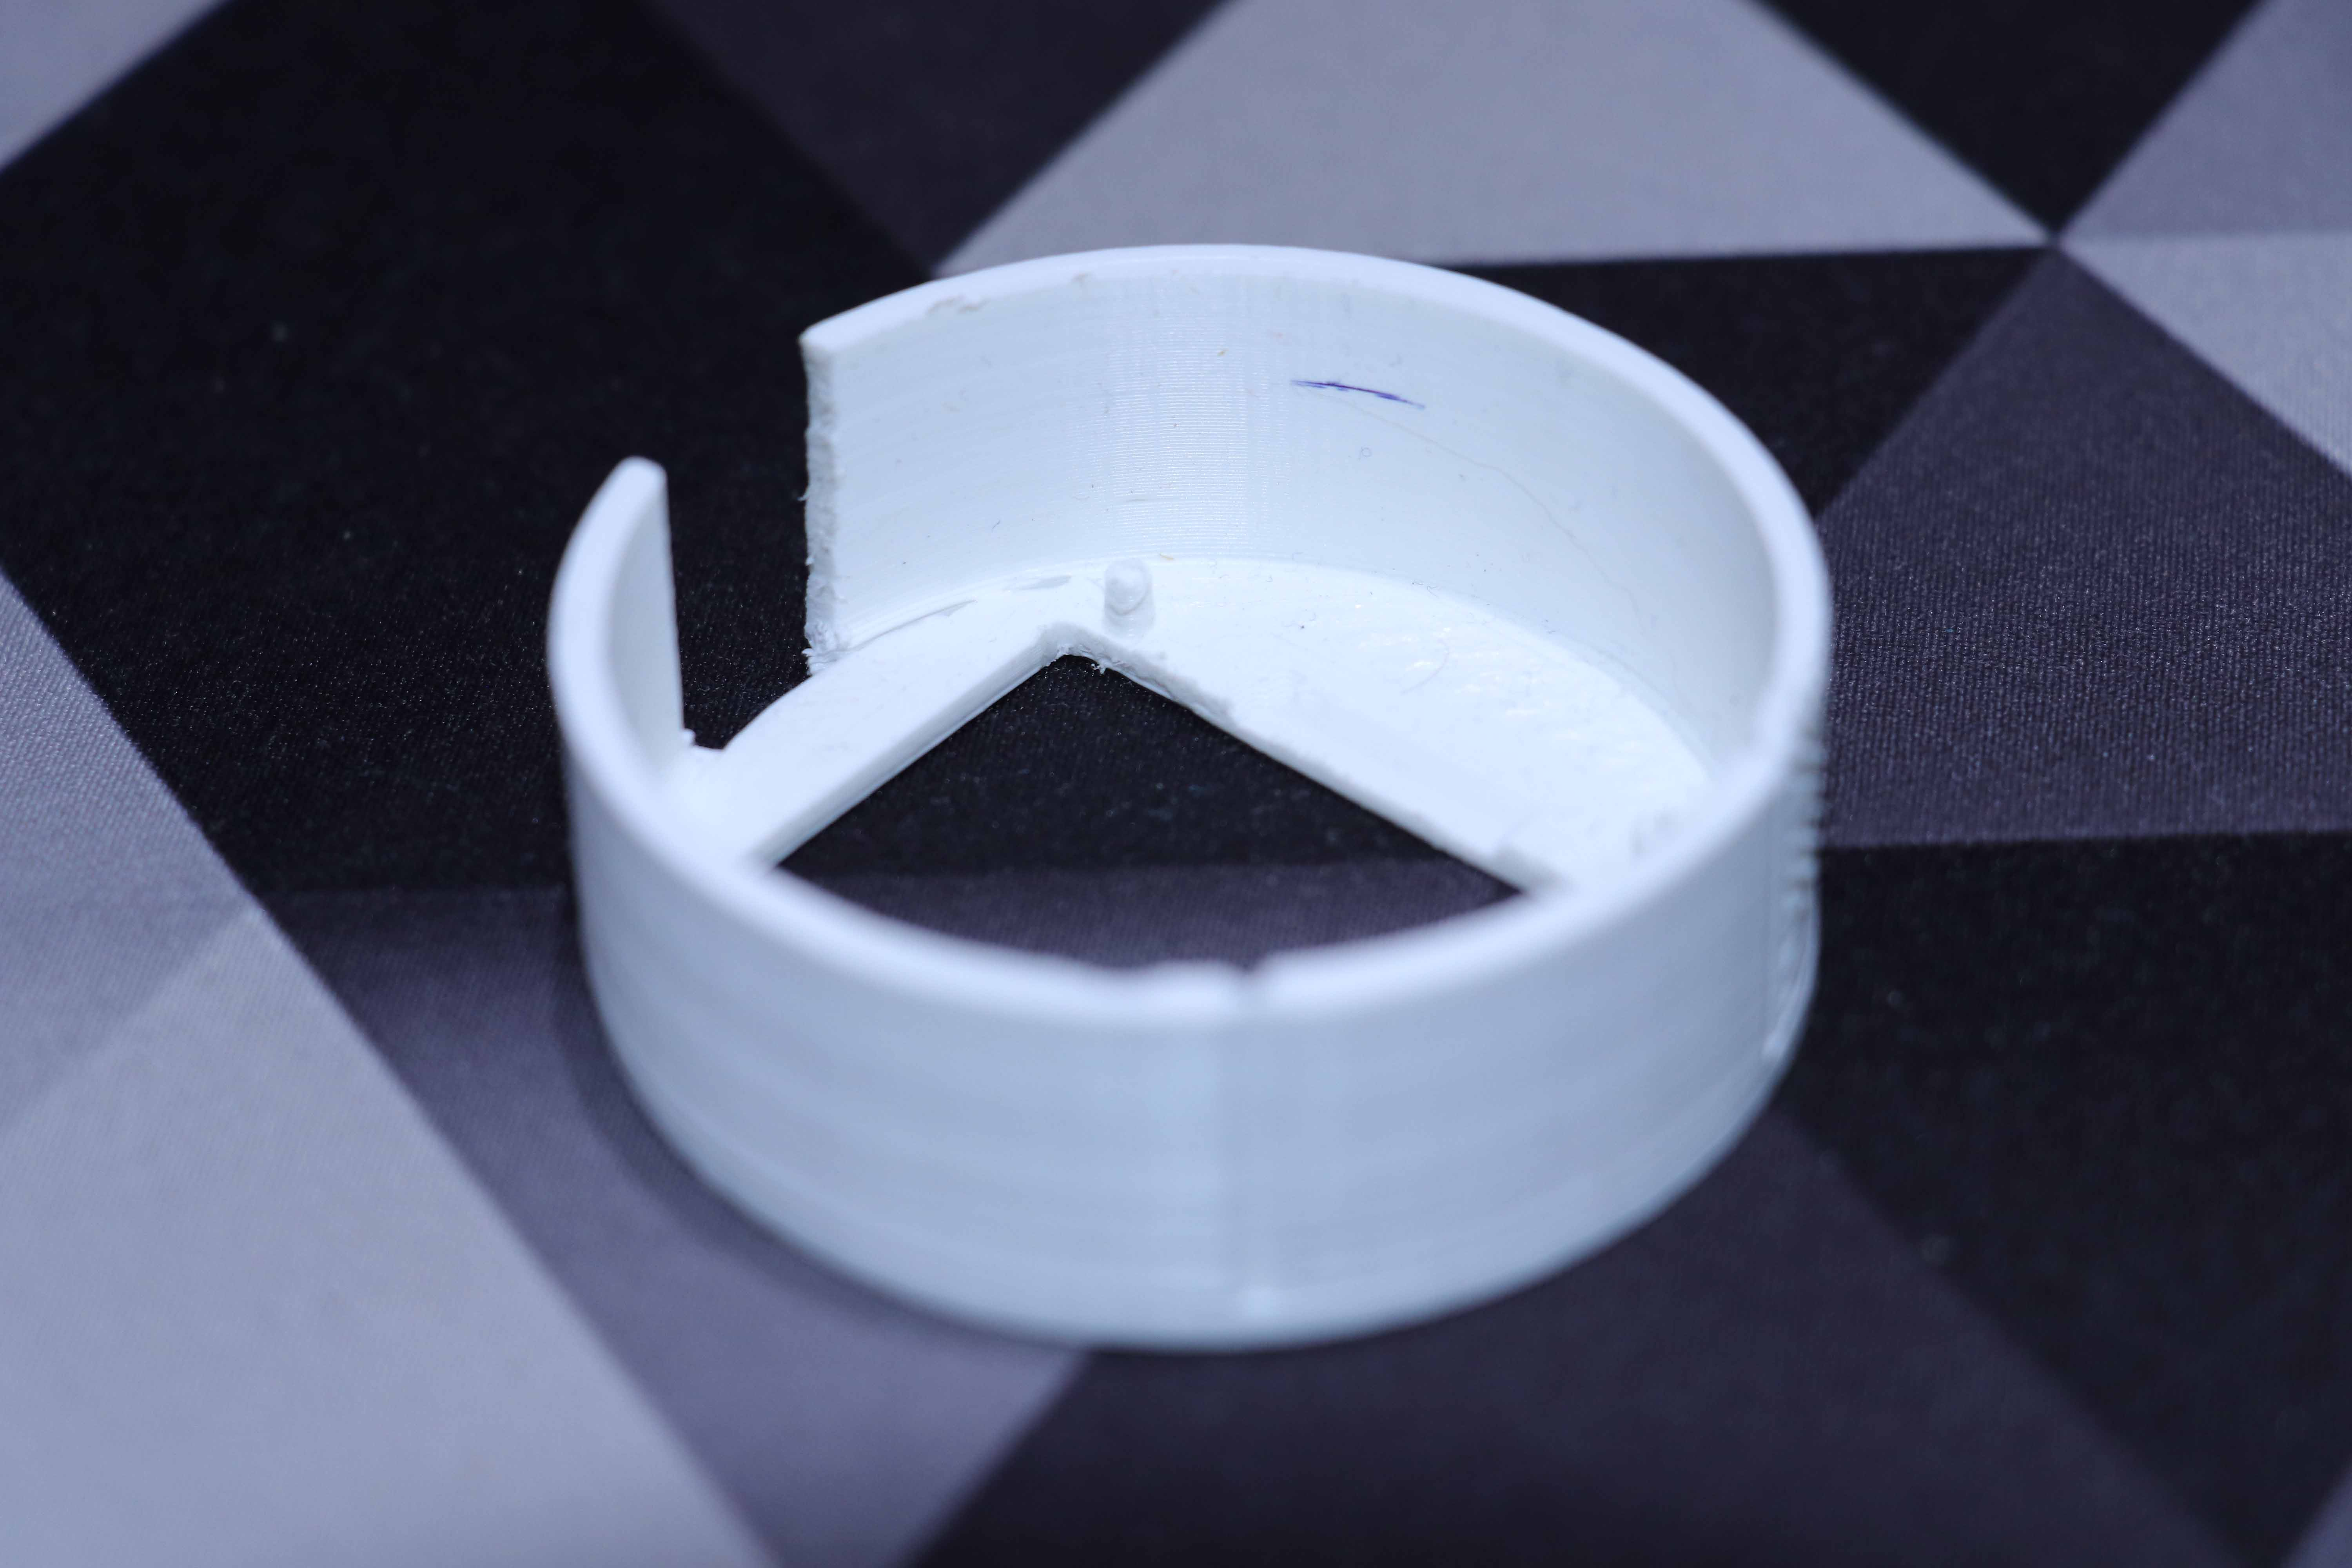
\includegraphics[width=\linewidth]{body_main_v1_back}
		\caption{نمای پشت}
		%\label{fig:oled_image}
	\end{subfigure}
	\begin{subfigure}{0.44\textwidth}
		\centering
		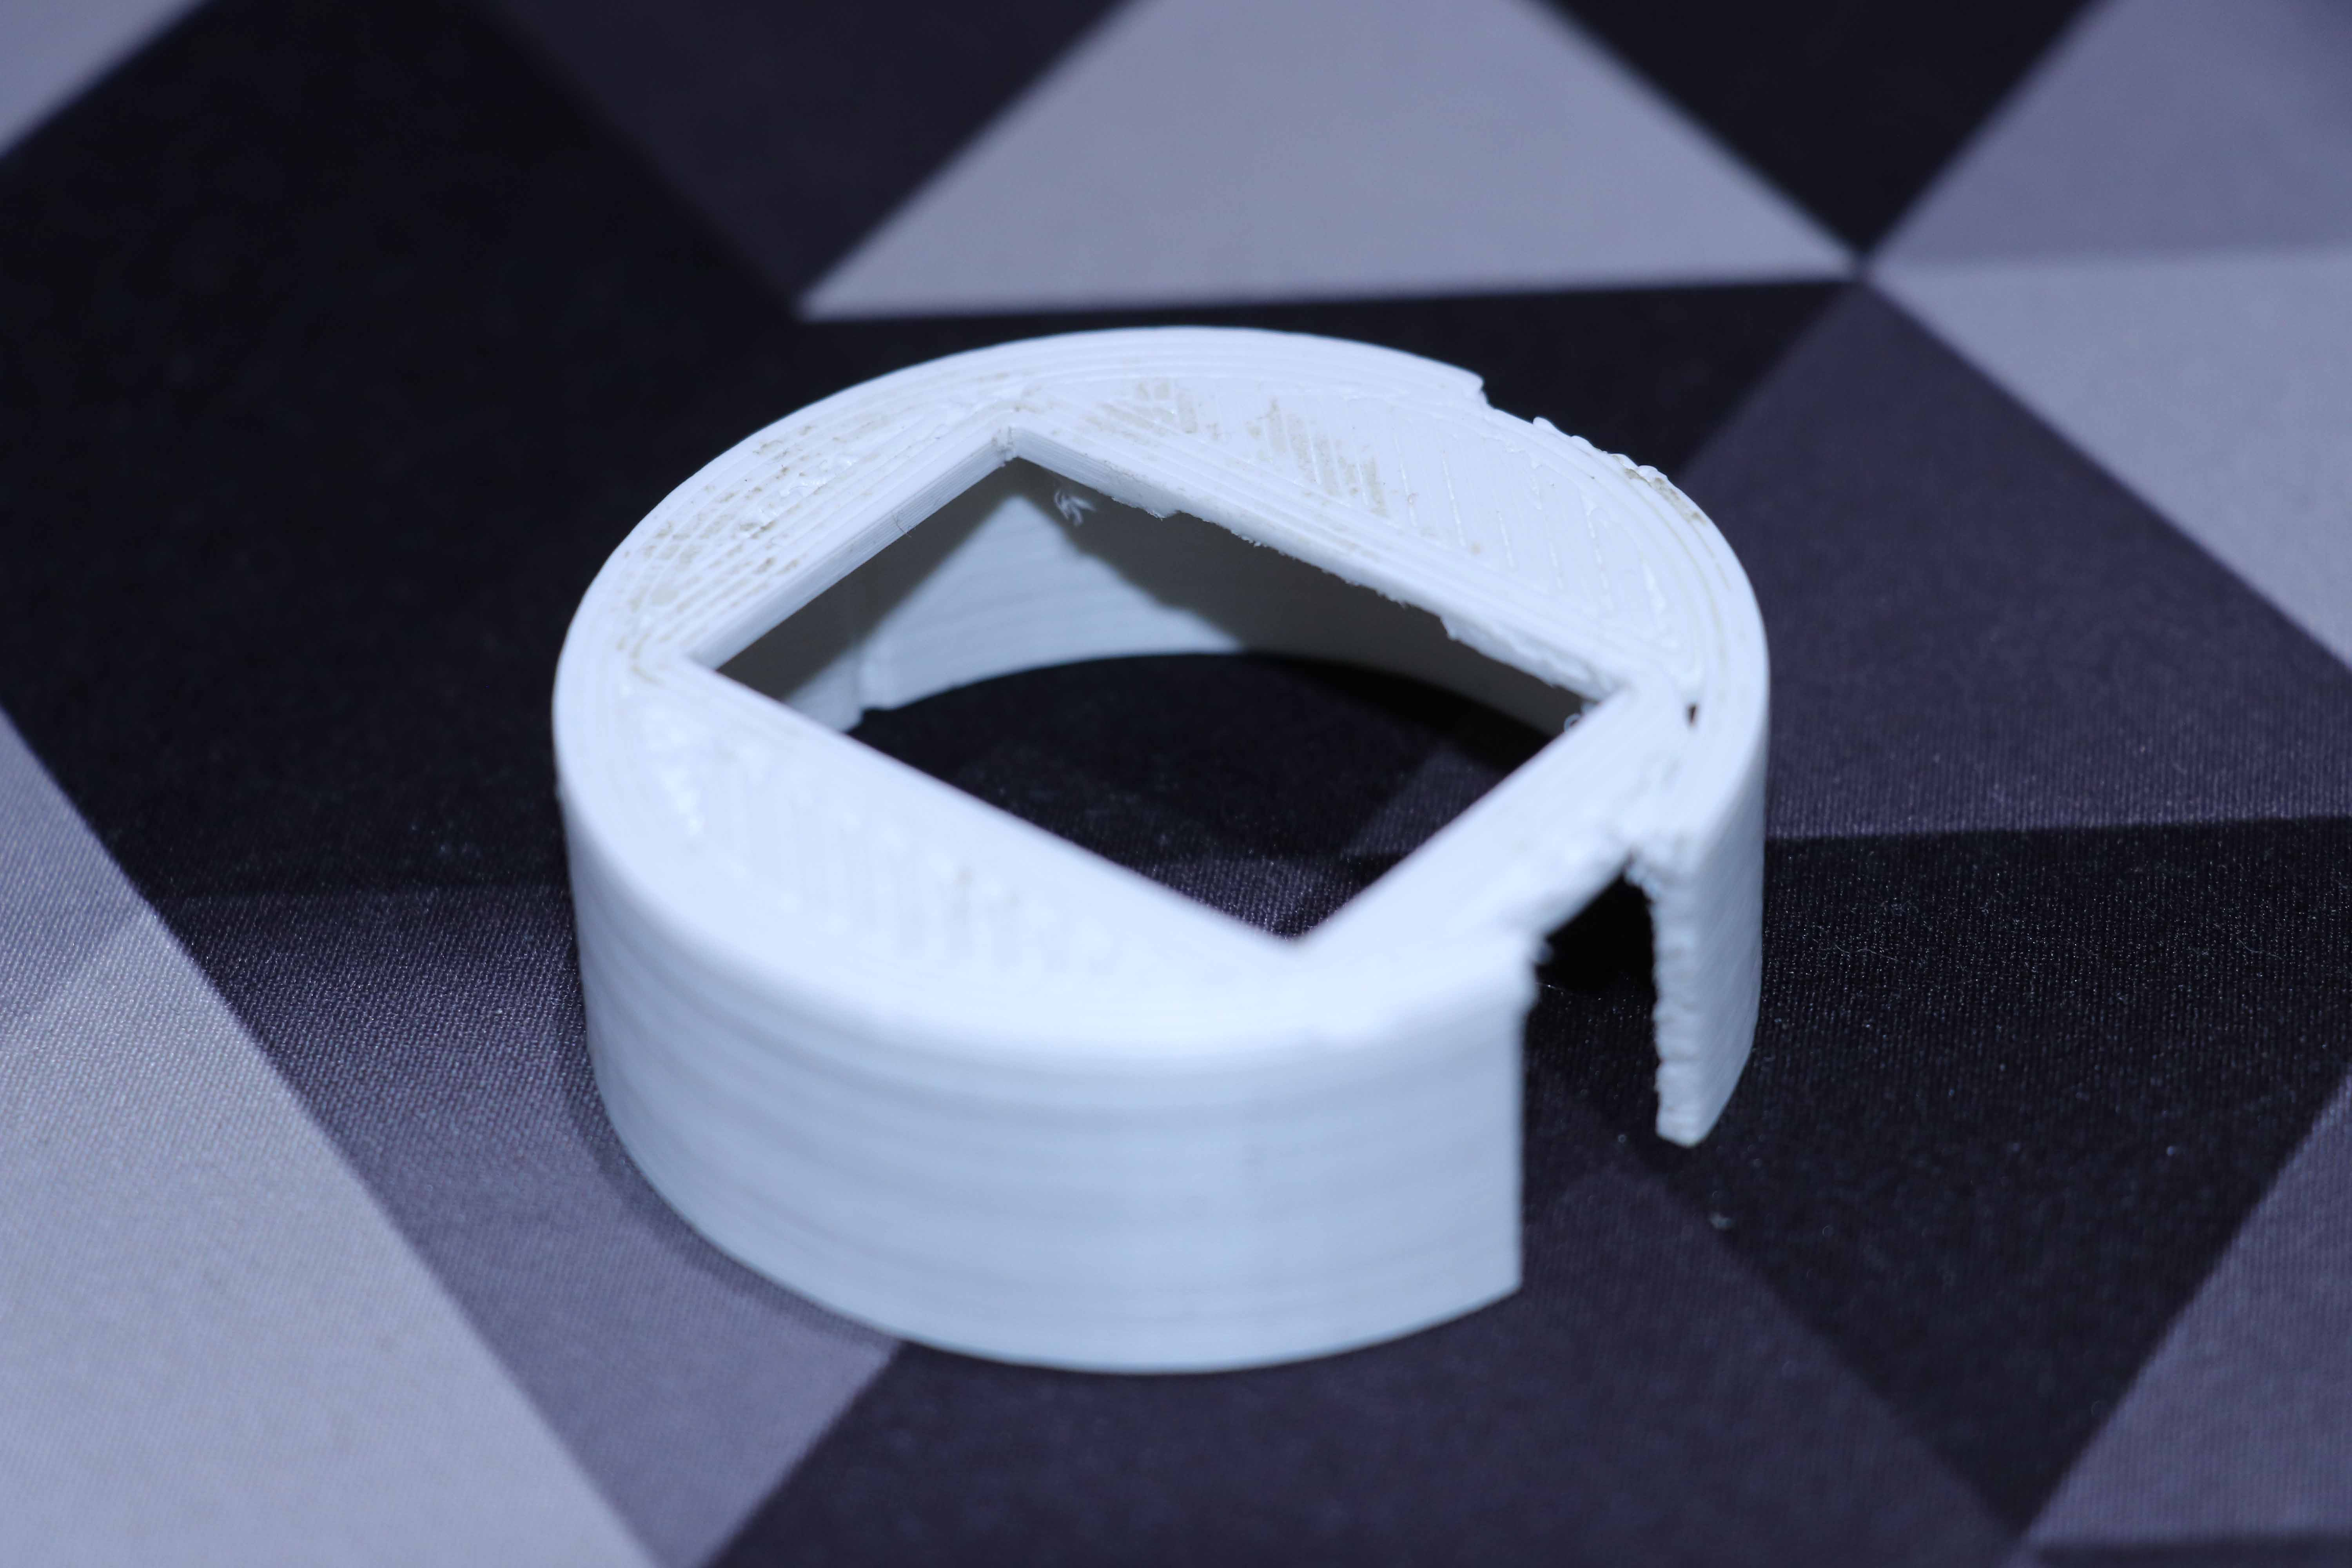
\includegraphics[width=\linewidth]{body_main_v1_front}
		\caption{نمای روبرو}
		%\label{fig:oled_real}
	\end{subfigure}
	\caption{تصاویر بدنه‌ی اصلی نسخه‌ی اول}
	\label{fig:body-v1}
\end{figure}

سپس بعد از نهایی شدن طرح کلی، جزئیات طرح تکمیل شد و نسخه‌ی دوم بدنه به چاپ رسید. تصویر این نسخه در شکل ؟ دیده می‌شود.

\begin{figure}[h]
	\centering
	\begin{subfigure}{0.44\textwidth}
		\centering
		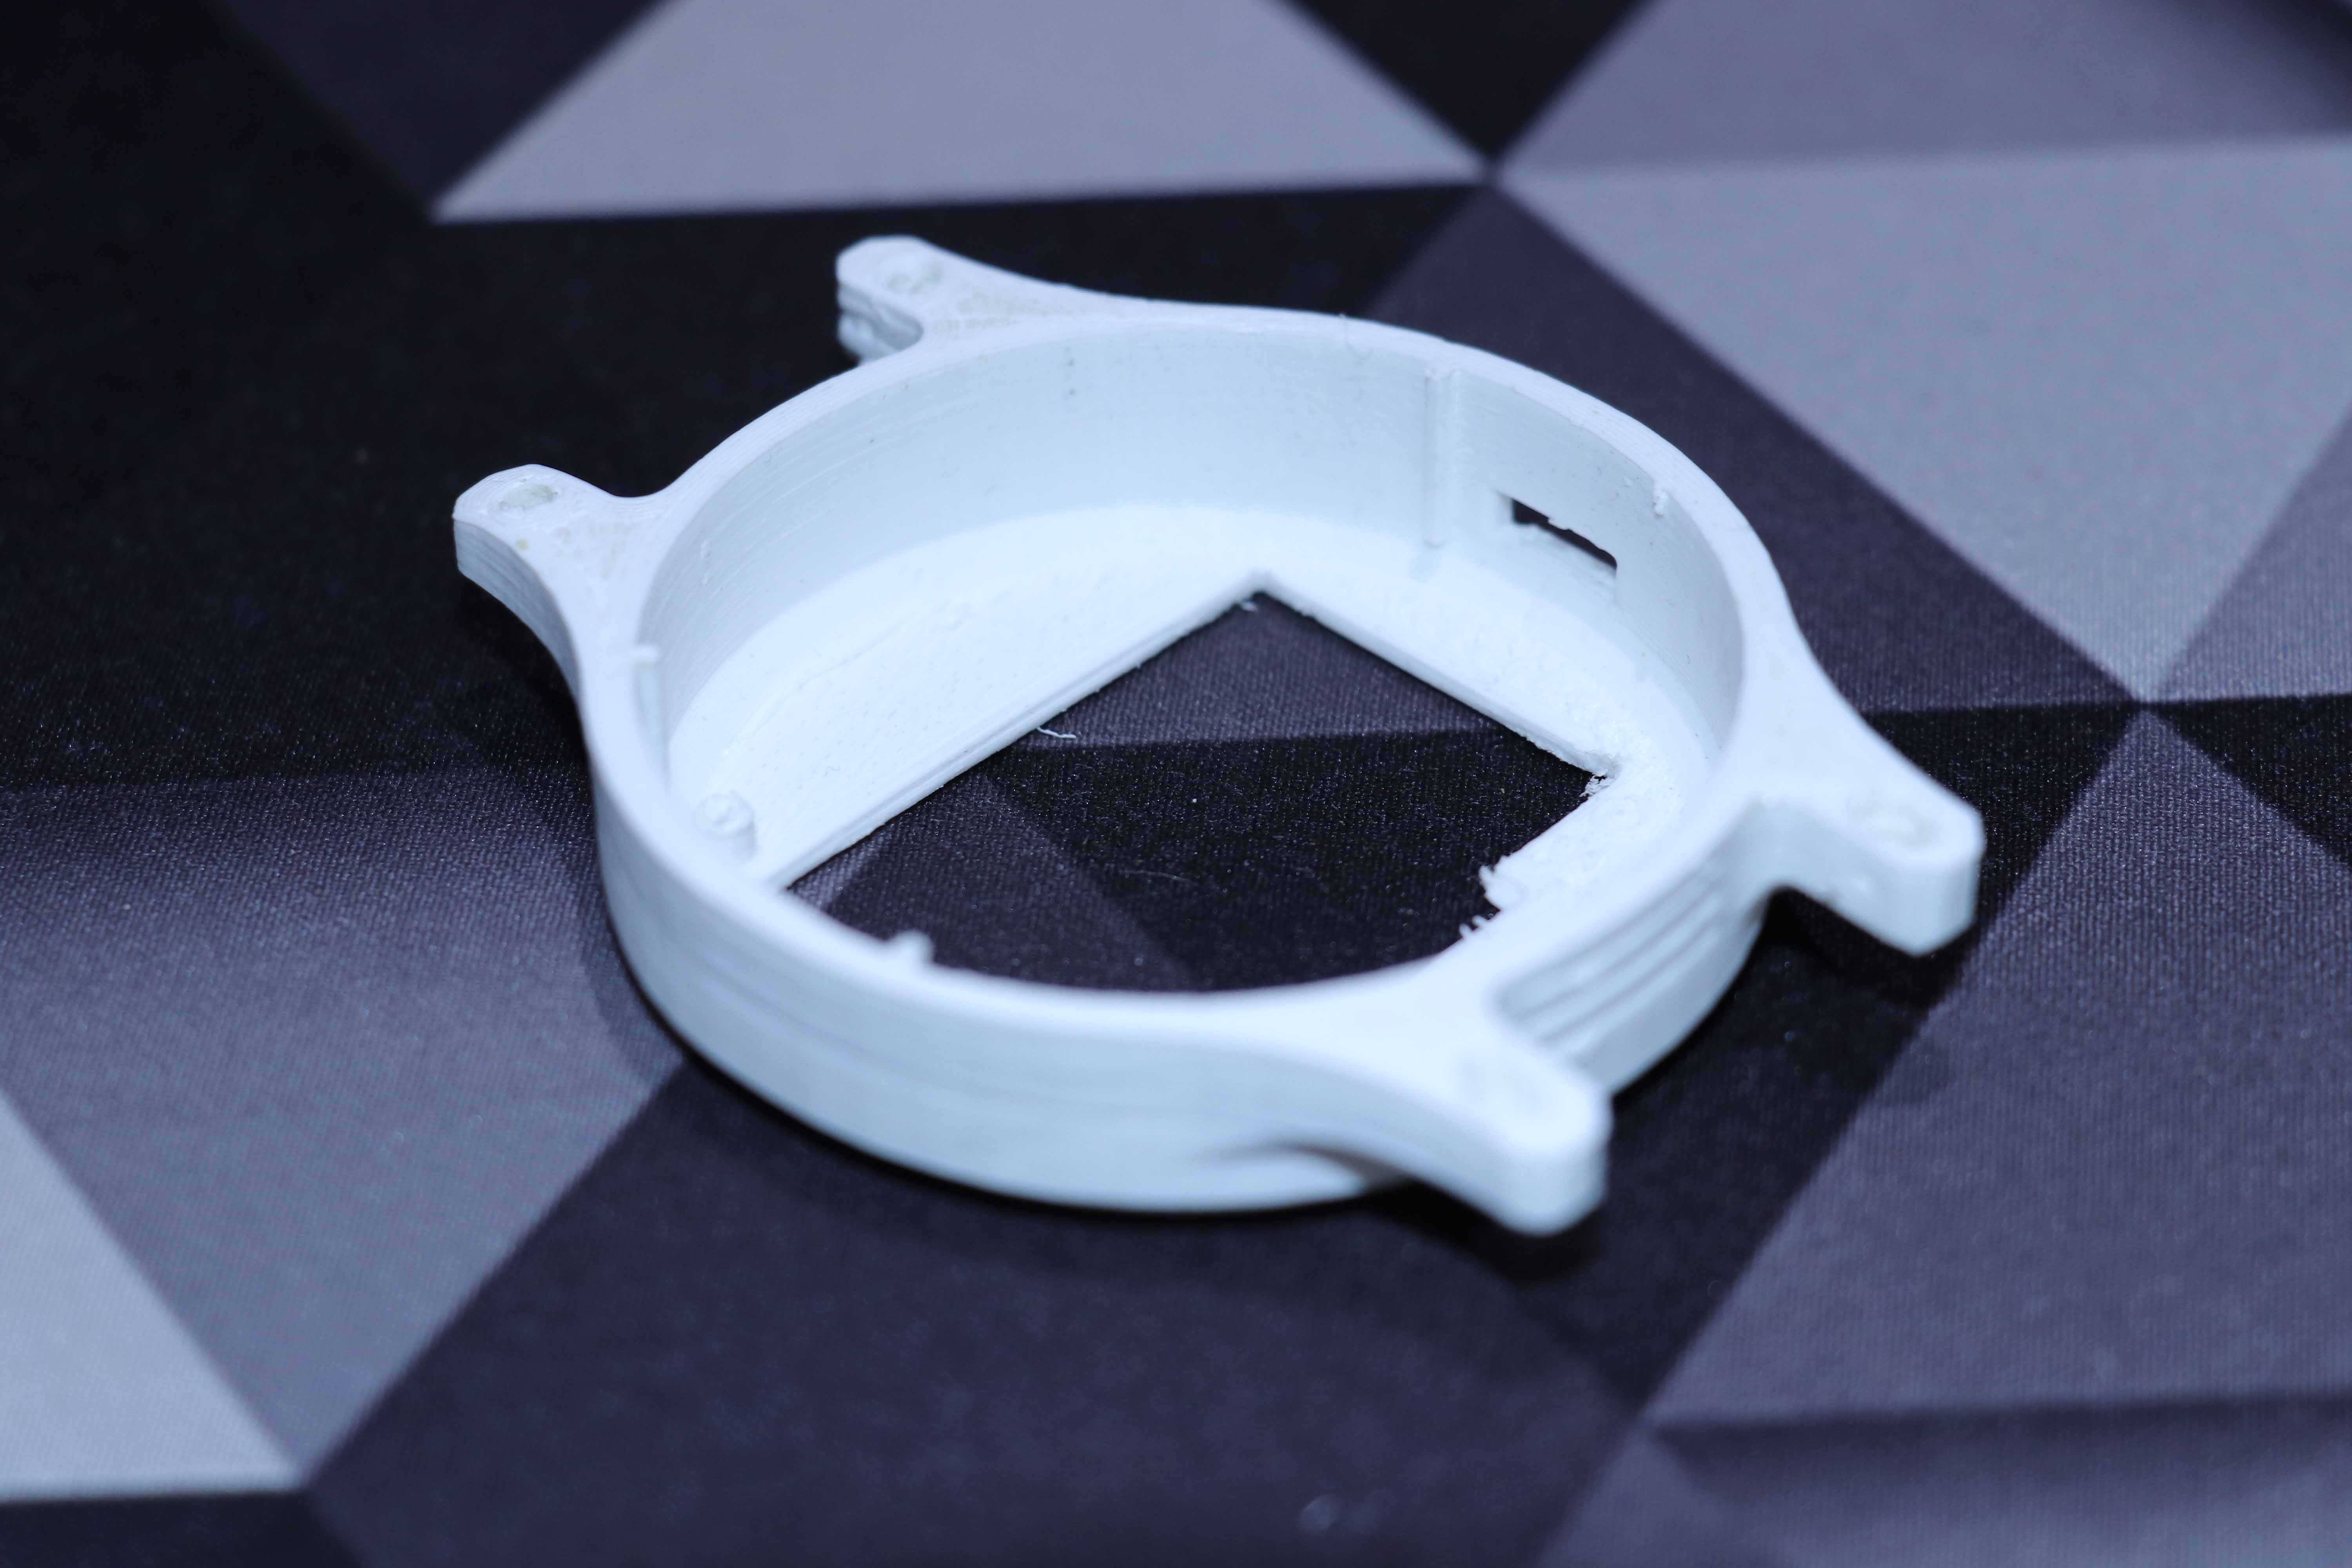
\includegraphics[width=\linewidth]{body_main_v2_back}
		\caption{نمای پشت}
		%\label{fig:oled_image}
	\end{subfigure}
	\begin{subfigure}{0.44\textwidth}
		\centering
		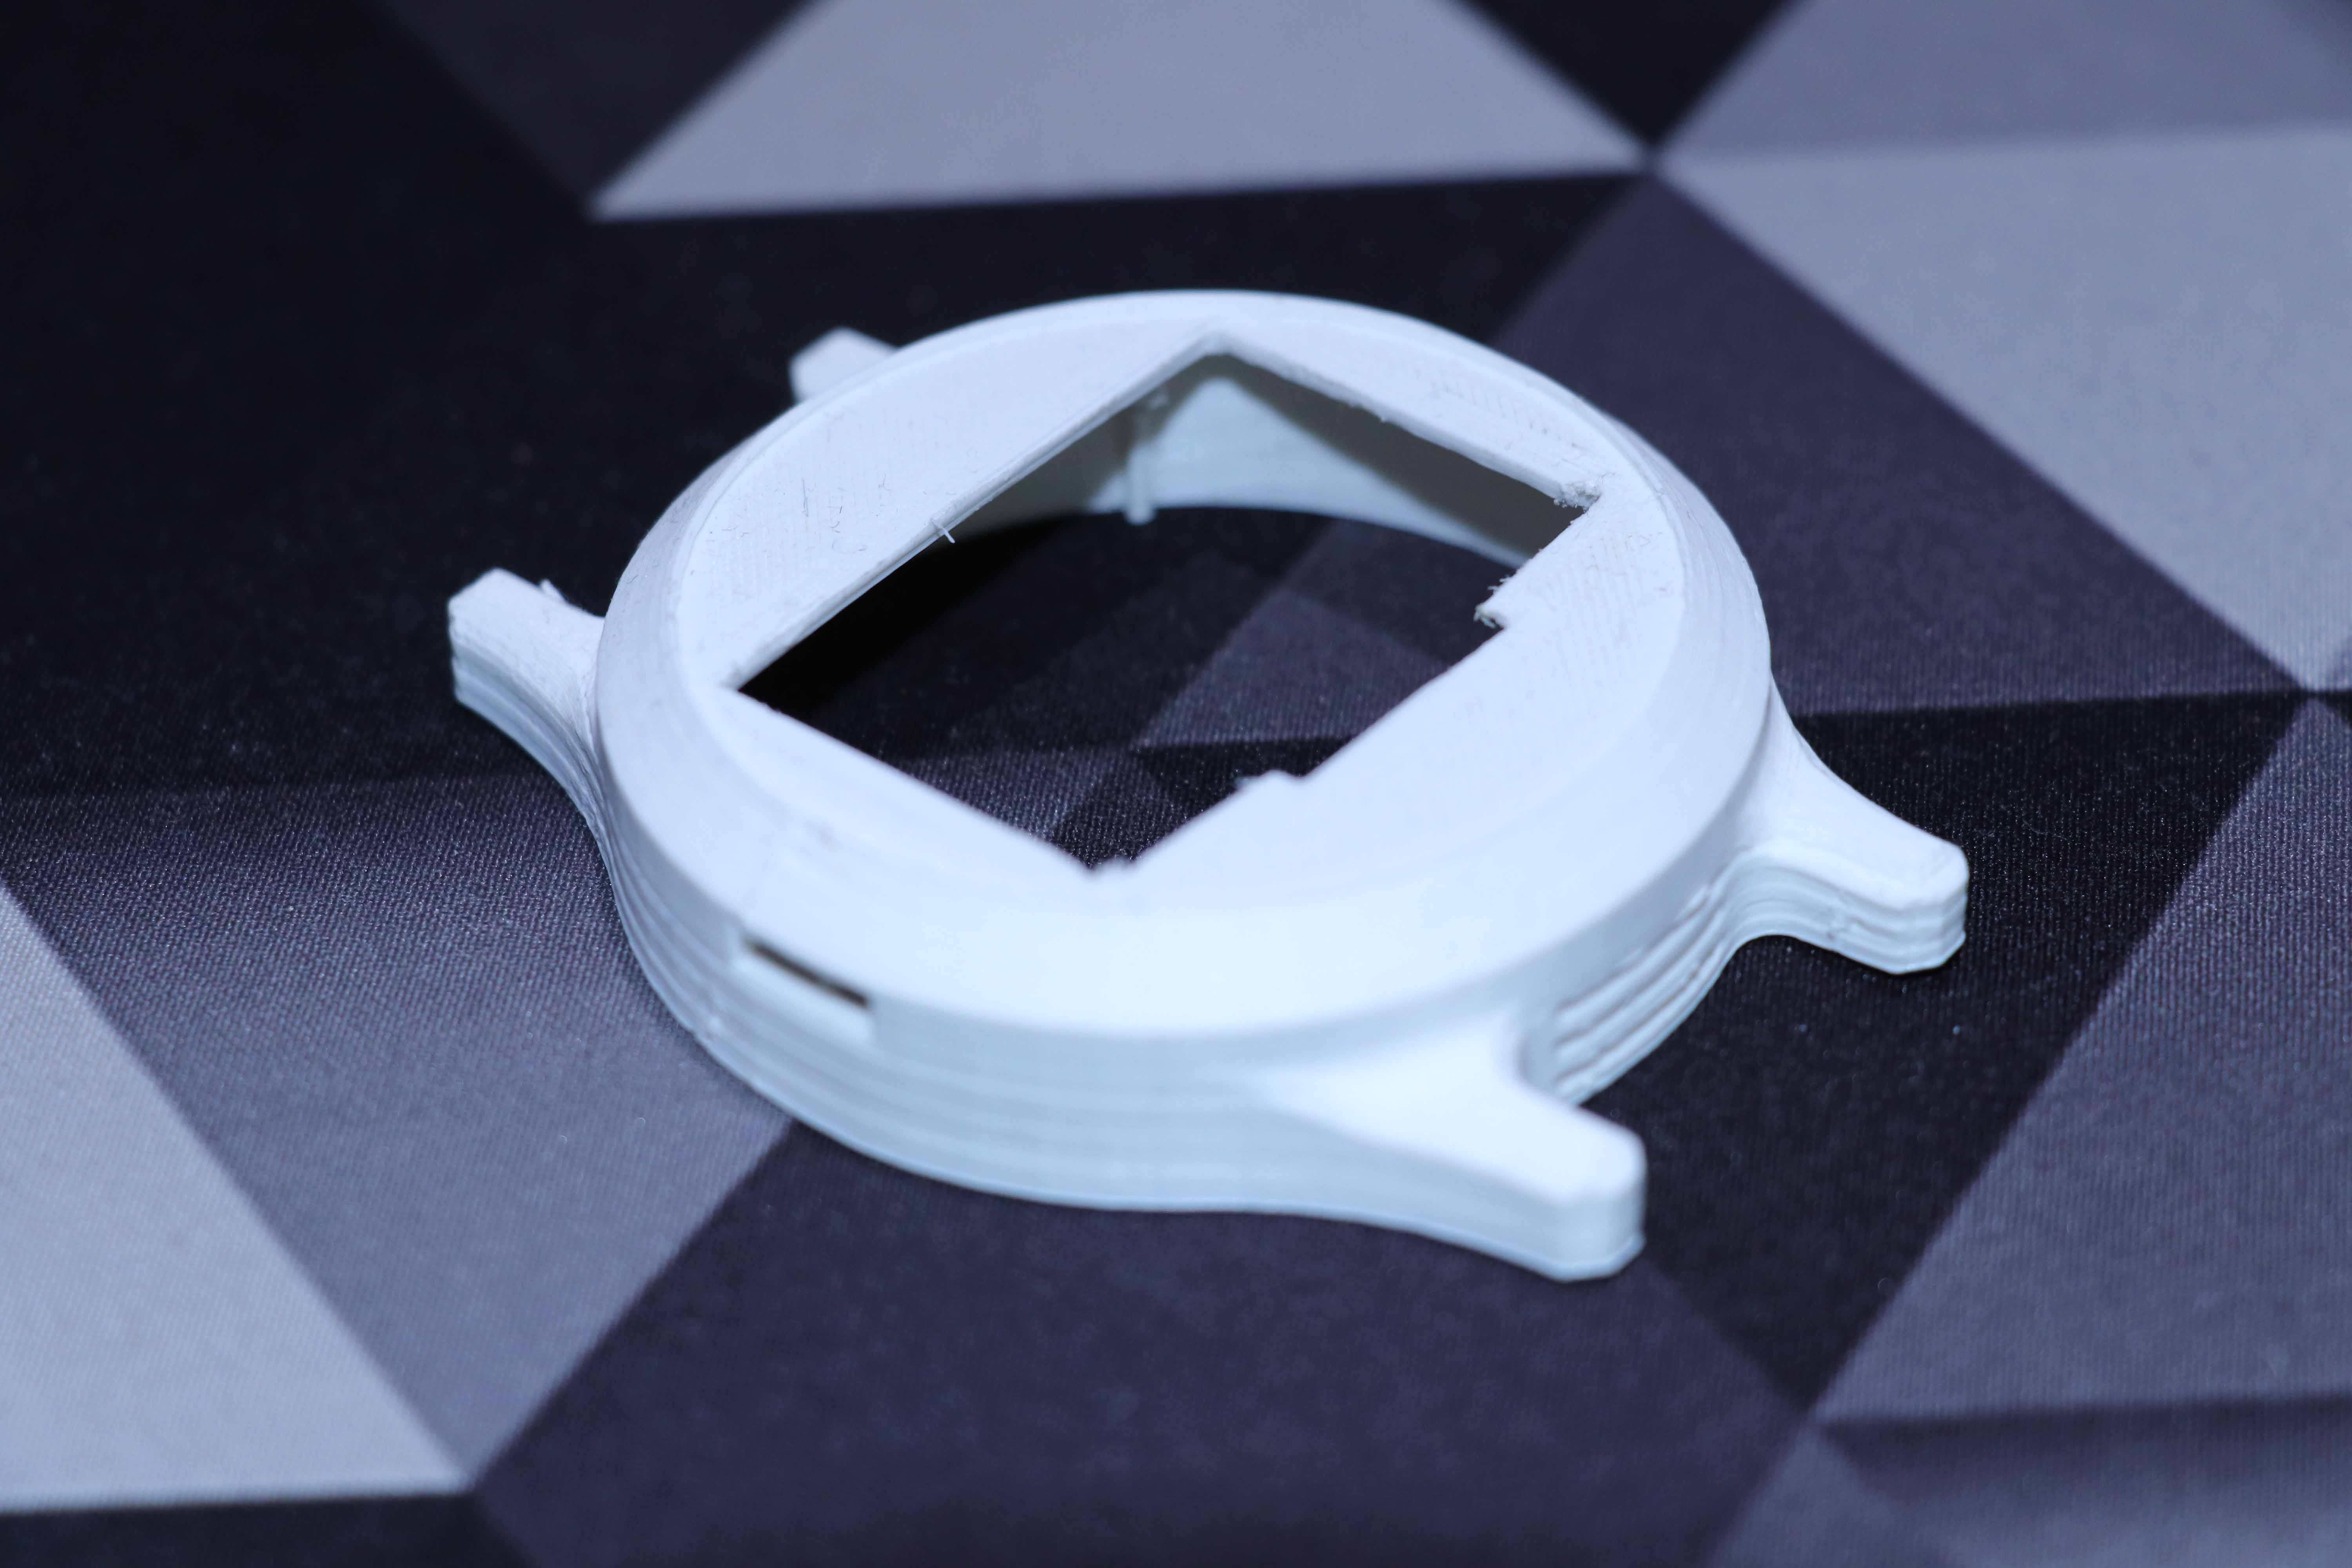
\includegraphics[width=\linewidth]{body_main_v2_front}
		\caption{نمای روبرو}
		%\label{fig:oled_real}
	\end{subfigure}
	\caption{تصاویر بدنه‌ی اصلی نسخه‌ی دوم}
	\label{fig:body-v2}
\end{figure}

این نسخه ایراداتی داشت، از جمله اینکه قسمت مربوط به محل اتصال بند بیش از حد بزرگ بود از زیبایی بصری می‌کاهید. بعد از برطرف نمودن ایرادات این نسخه، نسخه‌ی سوم به چاپ رسید که شکل ؟ آن را نشان می‌دهد.

\begin{figure}[h]
	\centering
	\begin{subfigure}{0.44\textwidth}
		\centering
		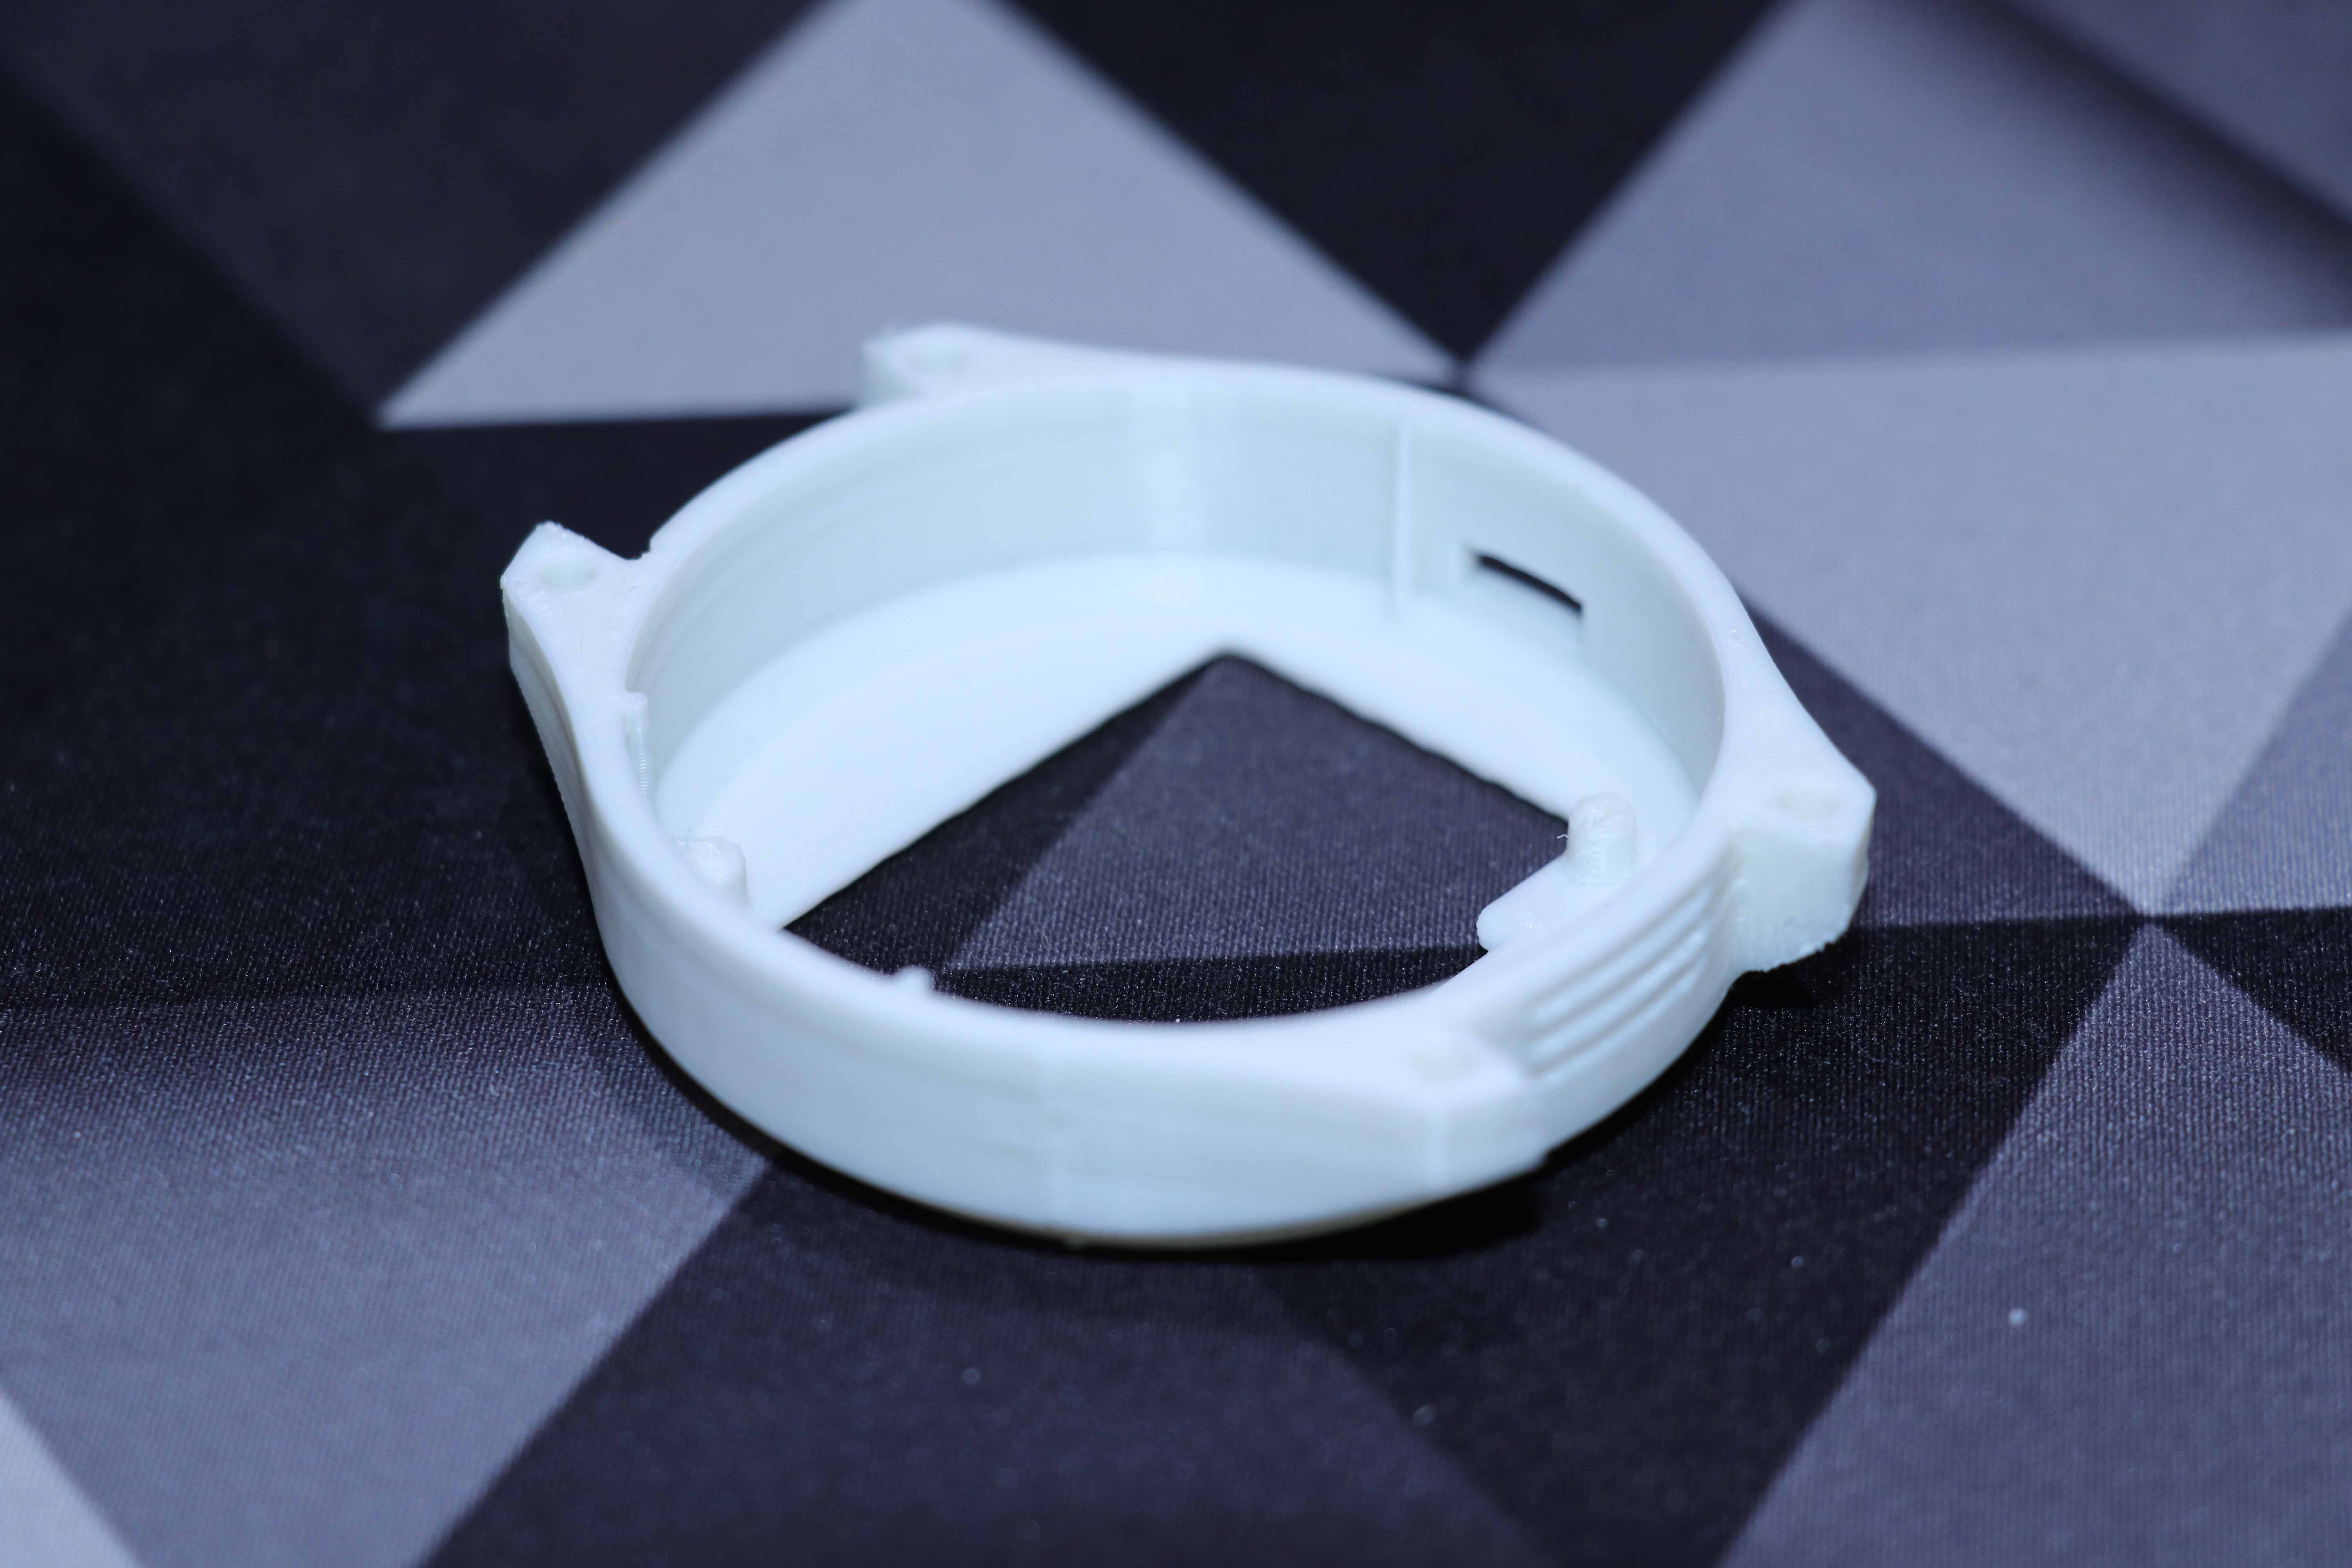
\includegraphics[width=\linewidth]{body_main_v3_back}
		\caption{نمای پشت}
		%\label{fig:oled_image}
	\end{subfigure}
	\begin{subfigure}{0.44\textwidth}
		\centering
		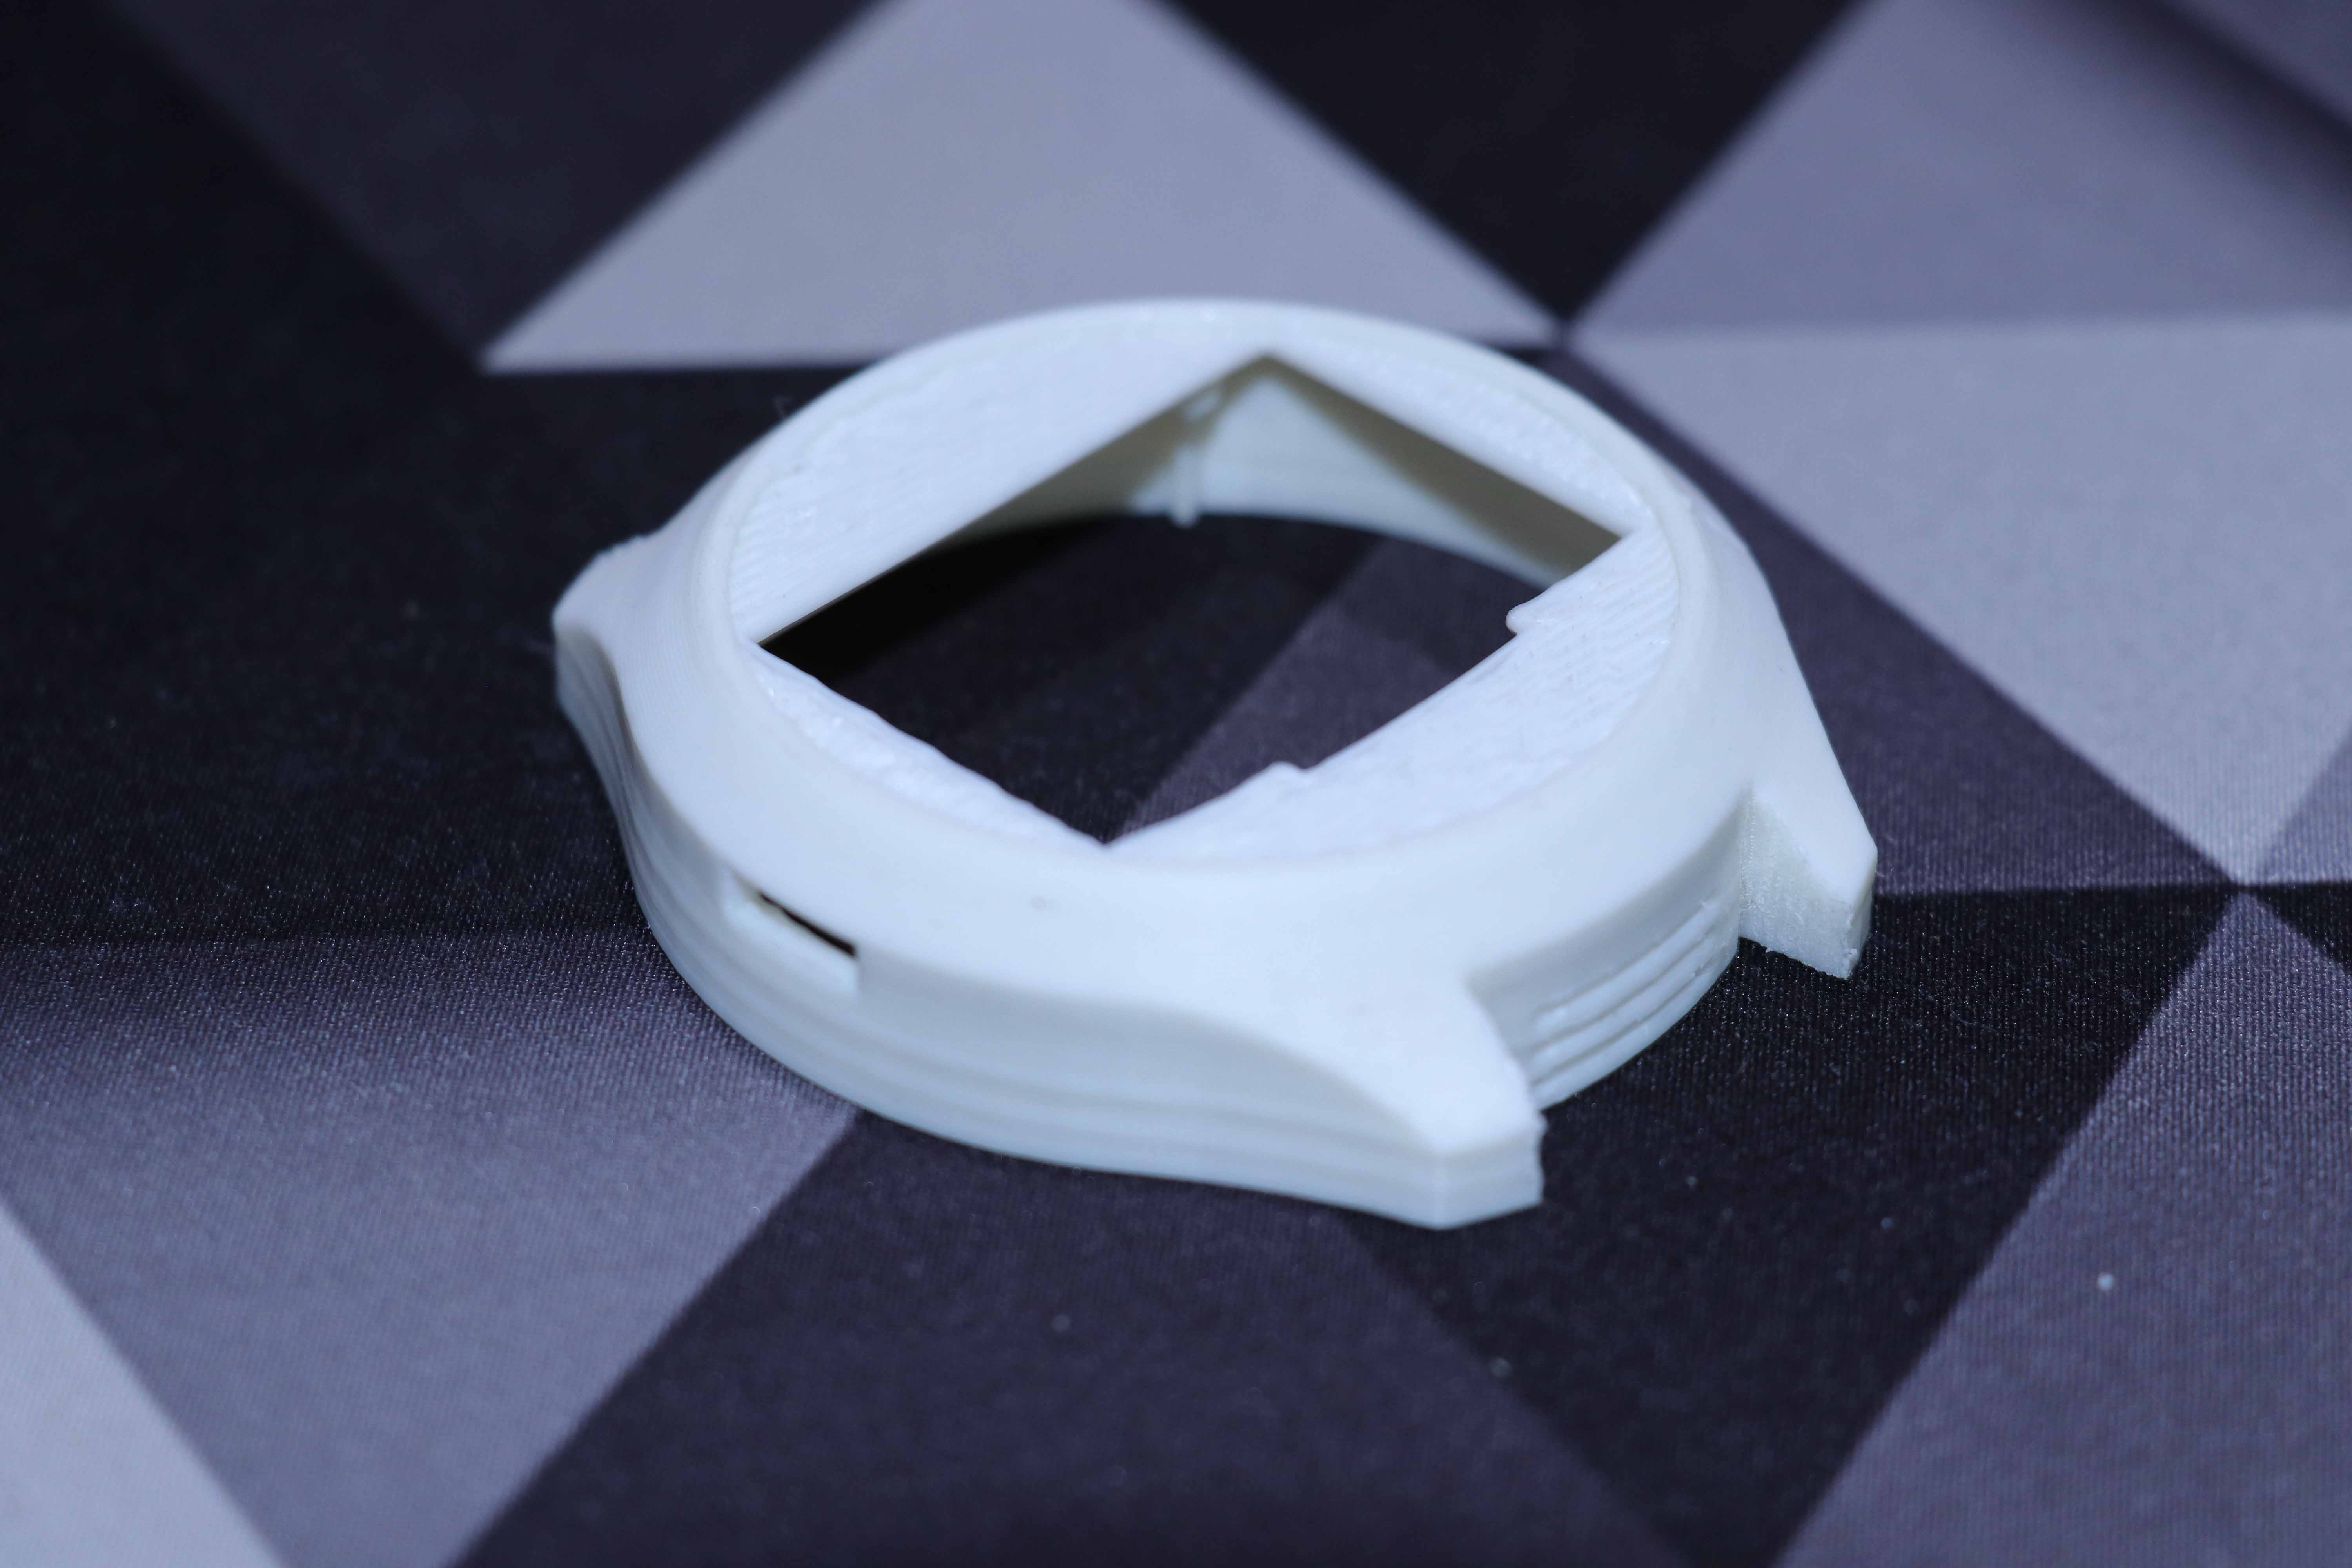
\includegraphics[width=\linewidth]{body_main_v3_front}
		\caption{نمای روبرو}
		%\label{fig:oled_real}
	\end{subfigure}
	\caption{تصاویر بدنه‌ی اصلی نسخه‌ی سوم}
	\label{fig:body-v3}
\end{figure}

این نسخه تقریبا تمام شرایط فوق را ارضا می‌کرد. جانمایی حسگر \lr{PPG} تنها موردی بود که باید انجام میشد. بعد از افزودن این قسمت، نسخه‌ی چهارم و نهایی آماده شد.

\subsection{نسخه نهایی}

شروط بحث شده در بالا را برای نسخه‌ی نهایی بررسی می‌کنیم.
\begin{enumerate}
	\item محل نصب صفحه نمایش:\\
	از سمت بیرون یک مستطیل خالی شده است که تا صفحه نمایش در آن قرار گیرد. از داخل هم سه استوانه منطبق بر سه سوراخ صفحه نمایش وجود دارد تا آن را در جای خود نگه دارد. اگر به تصویر صفحه نمایش (شکل \ref{fig:oled_image}) دقت کنید، پایین آن زائده‌ای برای اتصال سیم‌های فلت به صفحه نمایش قرار دارد. این زائده به شکل یک برش مستطیلی کوچک از صفحه‌ی فوقانی بدنه جدا شده است. شکل \ref{fig:body-oled} این قسمت ها را به خوبی نشان می‌دهد.
	
	\begin{figure}[h]
		\centering
		\begin{subfigure}{0.4\textwidth}
			\centering
			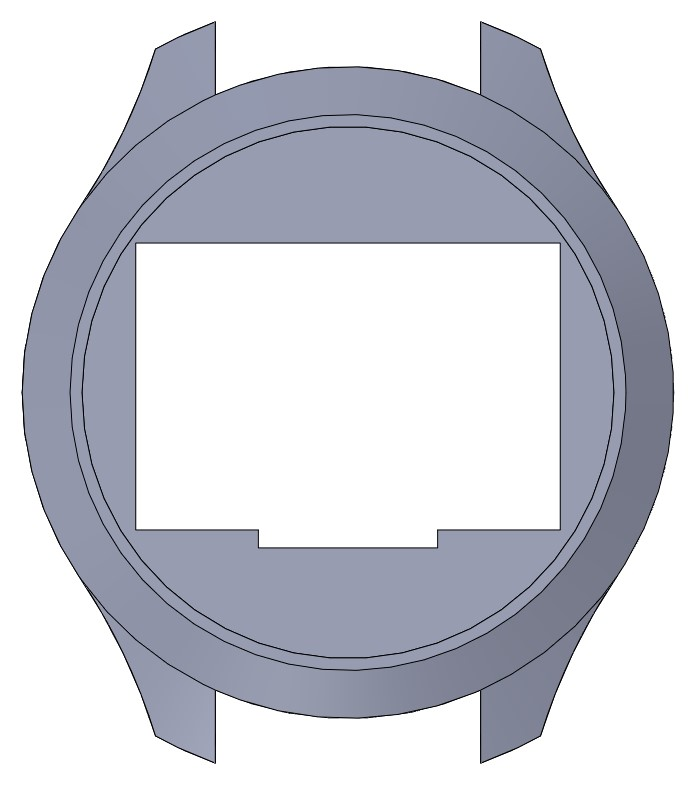
\includegraphics[width=0.78\linewidth]{body_oled}
			\caption{نمای درونی}
			%\label{fig:oled_image}
		\end{subfigure}
		\begin{subfigure}{0.45\textwidth}
			\centering
			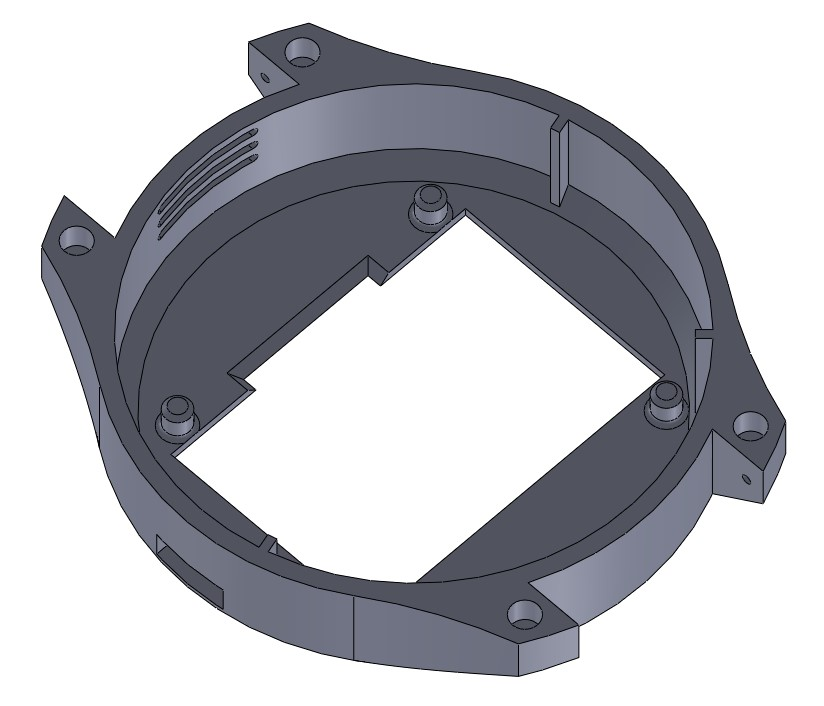
\includegraphics[width=\linewidth]{body_oled2}
			\caption{نمای بیرونی}
			%\label{fig:oled_real}
		\end{subfigure}
		\caption{تصاویر محل نصب صفحه نمایش در بدنه}
		\label{fig:body-oled}
	\end{figure}
	
	\item  جانمایی \pcbf و جلوگیری از چرخش آن:
	بر روی \pcbf سه شیار کوچک وجود دارد. متناظر با آن روی بدنه نیز سه زائده با همان ابعاد تعبیه شده است. این سه زائده مانع چرخش \pcbf در جای خود می‌شوند. تصویر این نگه‌دارنده‌ها در شکل ؟ قابل مشاهده است.
	
	\begin{figure}[h]
		\centering
		\begin{subfigure}{0.4\textwidth}
			\centering
			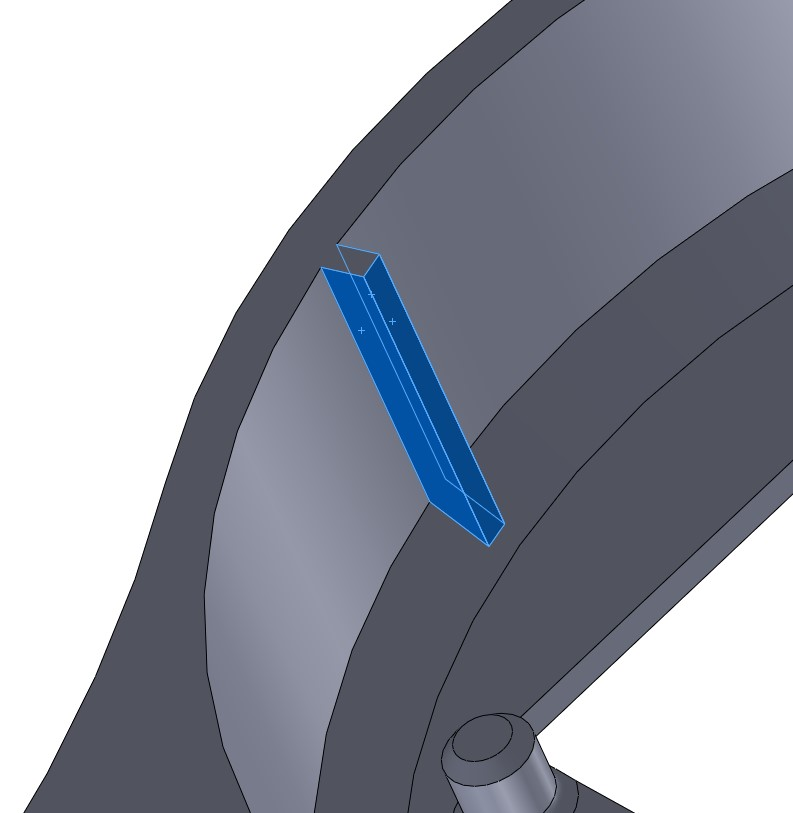
\includegraphics[width=\linewidth]{body_pcb2}
			\caption{نمای درونی}
			%\label{fig:oled_image}
		\end{subfigure}
		\begin{subfigure}{0.45\textwidth}
			\centering
			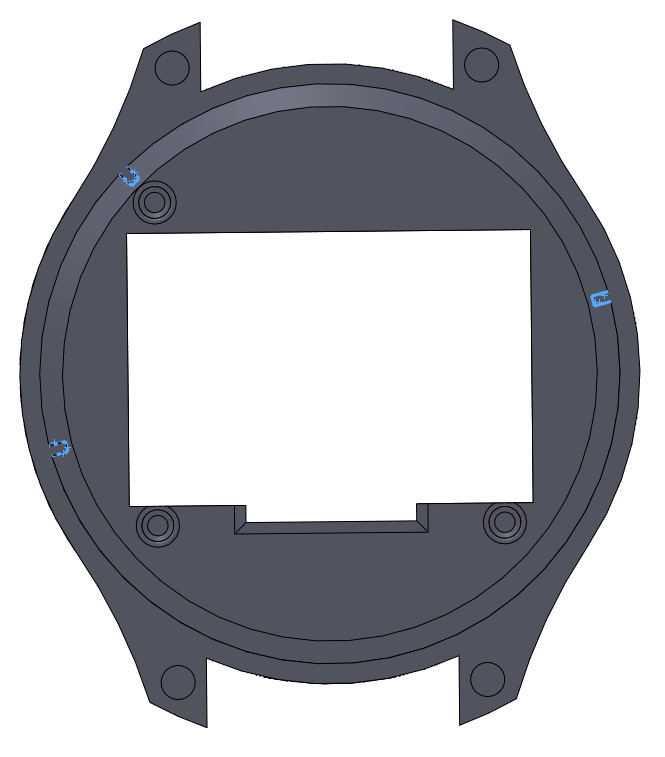
\includegraphics[width=\linewidth]{body_pcb}
			\caption{نمای بیرونی}
			%\label{fig:oled_real}
		\end{subfigure}
		\caption{تصاویر محل نصب \pcbf در بدنه}
		\label{fig:body-pcb}
	\end{figure}
	
	\item محل اتصال کابل \lr{USB}:
	بر سطح جانبی بدنه یک سوراخ مستطیل شکل به ابعاد کانکتور \lr{micro USB} تعبیه شده است. شکل \ref{fig:body-usb} محل آن روی بدنه را نمایش می‌دهد.

	\begin{figure}[h]
		\centering
		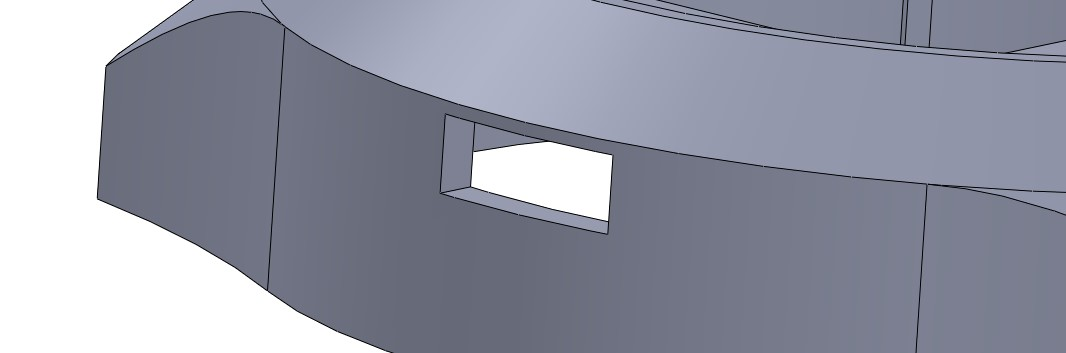
\includegraphics[width=0.9\linewidth]{body_usb}
		\caption{تصویر محل اتصال \lr{USB} در بدنه}
		\label{fig:body-usb}
	\end{figure}
	
	\item محل عبور هوا:
	در نزدیکی قطعات مدار شارژ سه شیار برای عبور هوا وجود دارد تا قطعات داخلی به علت بالا رفتن دما آسیب نبینند. این شیارها در شکل \ref{fig:body-air} قابل مشاهده‌اند.
	
	\begin{figure}[h]
		\centering
		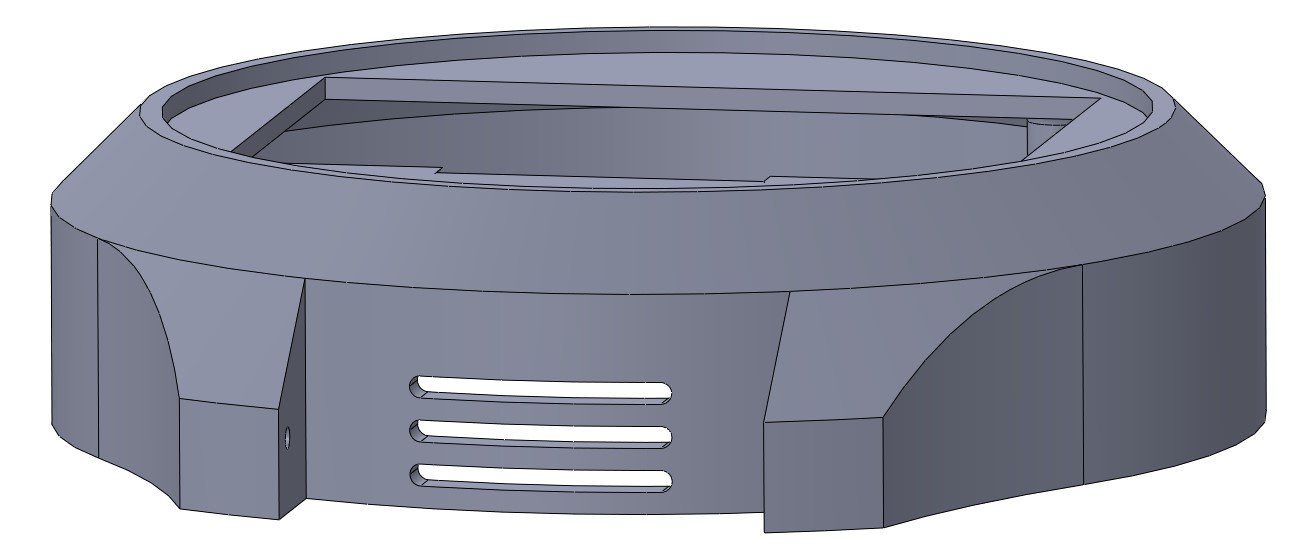
\includegraphics[width=0.9\linewidth]{body_air}
		\caption{تصویر شیارهای عبور هوا}
		\label{fig:body-air}
	\end{figure}

	\item محل اتصال بند
	بندهای موردنظر برای این ساعت مربوط به ساعت هوشمند \lr{Haylou} است. این بندها از جنس پلاستیک هستند. برای اتصال بند به بدنه‌ی اصلی چهار بازوی کوچک به بدنه اضافه شده است. داخل آن‌ها سوراخ‌هایی کوچکی موجود است که پین بند در آن‌ها قرار گیرد. تصویر این بازوها و محل نصب پین را شکل \ref{fig:body-band} مشاهده می‌کنید.
	
	\begin{figure}[h]
		\centering
		\begin{subfigure}{0.4\textwidth}
			\centering
			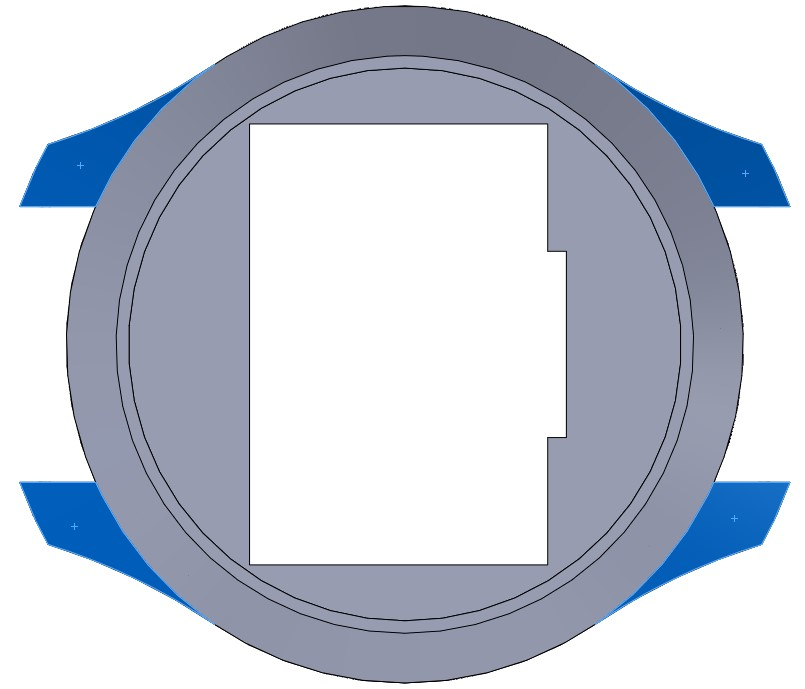
\includegraphics[width=\linewidth]{body_band}
			\caption{چهار بازو برای اتصال بند}
			%\label{fig:oled_image}
		\end{subfigure}
		\begin{subfigure}{0.3\textwidth}
			\centering
			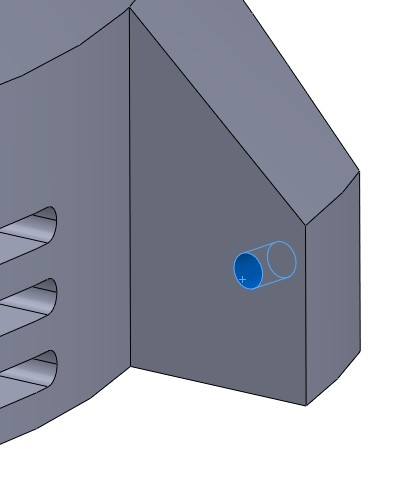
\includegraphics[width=\linewidth]{body_band2}
			\caption{سوراخ های نصب پین}
			%\label{fig:oled_real}
		\end{subfigure}
		\caption{تصاویر محل نصب بند}
		\label{fig:body-band}
	\end{figure}

	\item زیبایی بصری: جای تردید نیست که این طرح زیبا است :)
	\item ابعاد دقیق طرح در بخش‌های بعدی تشریخ خواهد شد؛ اما در مورد تناسب ابعاد، قطر دایره‌ی این ساعت حدود 5 سانتی‌متر است که در مقایسه با ساعت‌های موجود در بازار، مقدار بزرگی نیست و معقول است.
\end{enumerate}


\section{دریچه‌ی پشتی}


\section{اتصالات}

